\documentclass{betterposter}

\definecolor{st}{RGB}{214, 39, 20}
\renewcommand{\maincolumnbackgroundcolor}{st}

\begin{document}
    \betterposter{
    % Main column
        \maincolumn {
            \textbf{Machine Learning} algorithms
            show promise in \textbf{designing better
            riboswitches} for the
            \textbf{detection of dopamine}
        }{
            \compactqrcode{assets/repo-qr.png}{
                \textbf{Take a picture} to see \\ the Open-Source GitHub
            }
        }
    }{
    % Left column
        \title{ADAPT in SC ML in Synth Bio}
        \author{James Craven}
        \author{Matthew Lindsey}
        \institution{Winthrop University}

        \section{Introduction}
        Dopamine is important in:
        \begin{itemize}
            \item Addiction
            \item Mental Illnes
            \item Neurodegenerative Disorders
        \end{itemize}
        Designing sensors is costly, machine learning
        can speed it up\textellipsis

        \section{Methodologies}
        Inspired by Angenent-Mari et al. (2019), we
        attempted the following:
        \begin{itemize}
            \item Verify that training on the the
            sequences of RNA themselves would perform
            better
            \item Build an architecture to train future
            models
            \item Attempt to cross-train pre-existing
            models on WU's data
        \end{itemize}

        \vspace{5in}
        \begin{center}
            \includegraphics[width=0.9\linewidth]{assets/Unit Signature-Mathematics_black-stack.png}
        \end{center}
    }{
    % Right column

        \section{Results}
        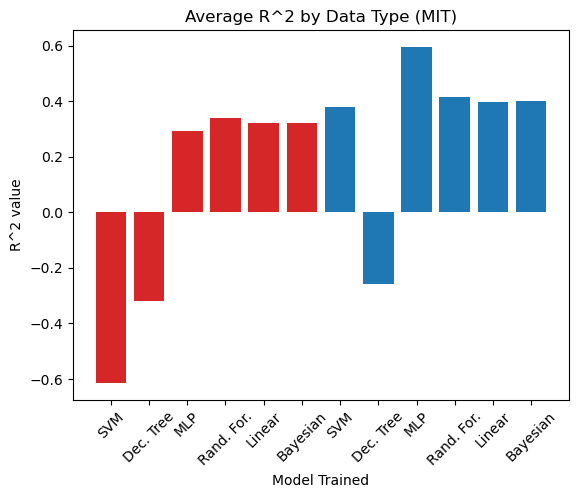
\includegraphics{assets/Average-R^2-by-Data-Type-MIT.png}
        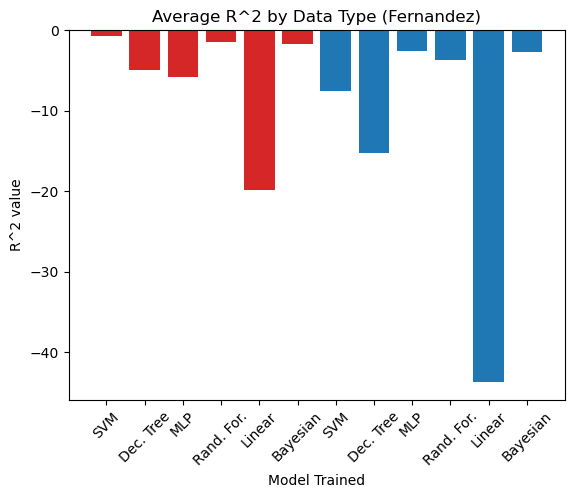
\includegraphics{assets/Average-R^2-by-Data-Type-Fernandez.png}

        \section{Acknowledgements}
        
        This work was supported primarily by the National Science Foundation
        EPSCoR Program under NSF Award \#OIA-2242812. Any Opinions, findings
        and conclusions or recommendations expressed in this material are
        those of the author(s) and do not necessarily reflect those of the
        National Science Foundation.


    }
\end{document}